\documentclass{article}
\usepackage{tikz}
\begin{document}\

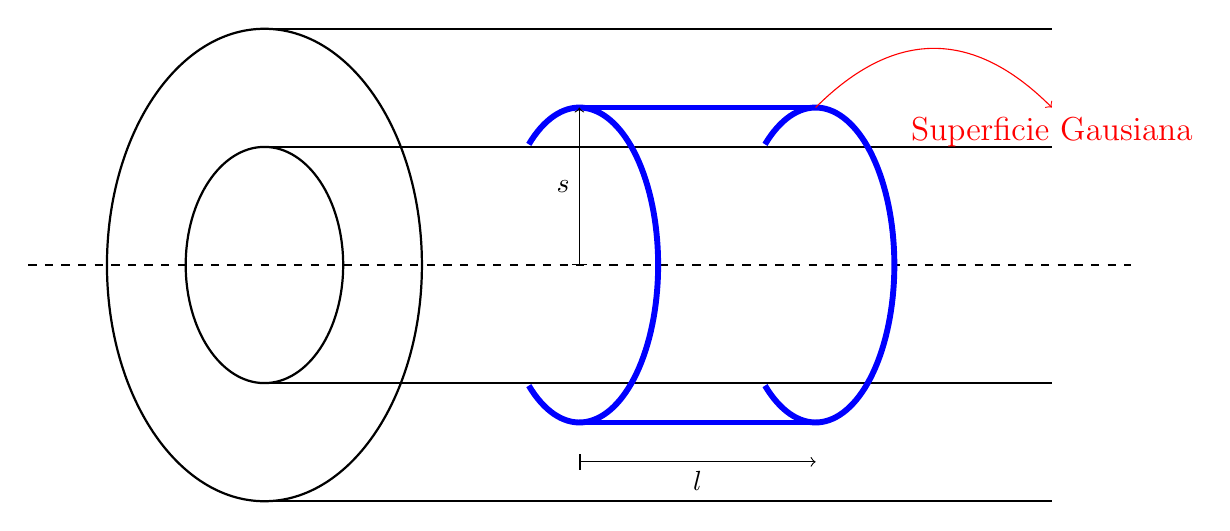
\begin{tikzpicture}
    % Outer cylinder (radius a)
    \draw[thick] (0,0) ellipse (2 and 3);
    \draw[thick] (0,0) ellipse (1 and 1.5);
    \draw[thick] (0,3) -- (10,3);
    \draw[thick] (0,1.5) -- (10,1.5);
    \draw[thick] (0,-1.5) -- (10,-1.5);
    \draw[thick] (0,-3) -- (10,-3);

    \draw[dashed](-3,0) -- (11,0);
    % cilindro de la parte interior 
    \draw[thick,blue, domain=130:-130, samples=100, variable=\t,line width=0.75mm] 
    plot ({1*cos(\t)+4}, {2*sin(\t)});
    
    \draw[thick,blue, domain=130:-130, samples=100, variable=\t,line width=0.75mm] 
    plot ({1*cos(\t)+7}, {2*sin(\t)});

    \draw[thick,line width=0.75mm,blue] (4,2) -- (7,2);
    \draw[thick,line width=0.75mm,blue] (4,-2) -- (7,-2);
    \draw[|->] (4,-2.5) -- (7,-2.5) node[midway,below] {$l$};
    \draw[|->,dash pattern=on 2pt off 0pt] (4,0) -- (4,2) node[midway,left] {$s$};

    \draw[->,red] (7,2) .. controls (8,3) and (9,3) .. (10,2) node[below,font = \large] {Superficie Gausiana};
\end{tikzpicture}

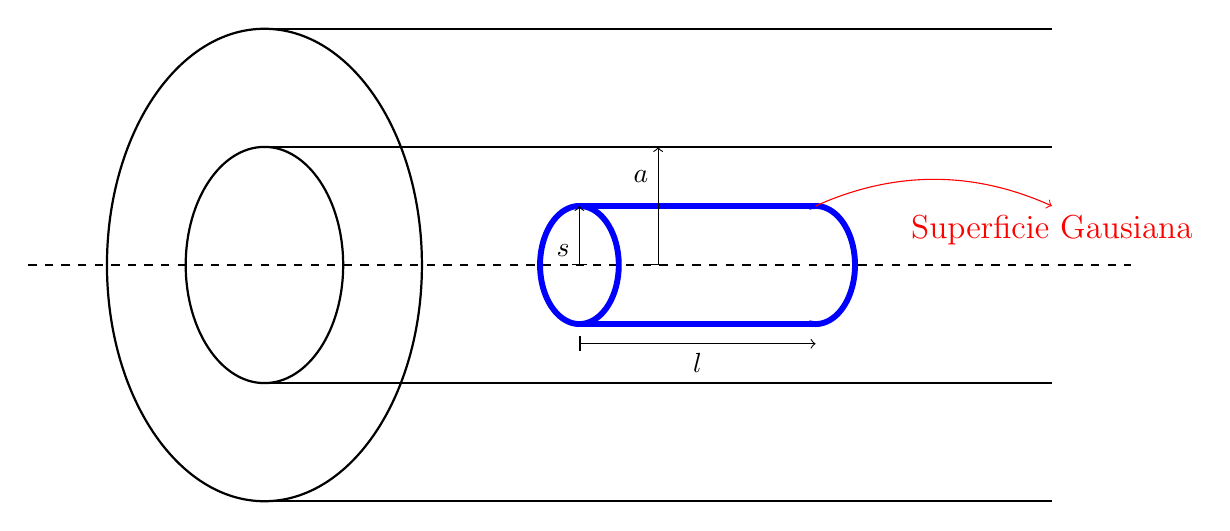
\begin{tikzpicture}
    % Outer cylinder (radius a)
    \draw[thick] (0,0) ellipse (2 and 3);
    \draw[thick] (0,0) ellipse (1 and 1.5);
    \draw[thick] (0,3) -- (10,3);
    \draw[thick] (0,1.5) -- (10,1.5);
    \draw[thick] (0,-1.5) -- (10,-1.5);
    \draw[thick] (0,-3) -- (10,-3);

    \draw[dashed](-3,0) -- (11,0);
    % cilindro de la parte interior 
    \draw[thick,blue ,domain = 0:360,samples=100, variable=\t,line width=0.75mm] 
    plot ({0.5*cos(\t)+4}, {0.75*sin(\t)});
    
    \draw[thick,blue,domain= 100:-100, samples=100, variable=\t,line width=0.75mm] 
    plot ({0.5*cos(\t)+7}, {0.75*sin(\t)});

    \draw[thick,line width=0.75mm,blue] (4,0.75) -- (7,0.75);
    \draw[thick,line width=0.75mm,blue] (4,-0.75) -- (7,-0.75);

\draw[|->] (4,-1) -- (7,-1) node[midway,below] {$l$};
    \draw[|->,dash pattern=on 2pt off 0pt] (4,0) -- (4,0.75) node[near start,left] {$s$};
    
    \draw[|->,dash pattern=on 2pt off 0pt] (5,0) -- (5,1.5) node[near end,left] {$a$};

    \draw[->,red] (7,0.75) .. controls (8,1.2) and (9,1.2) .. (10,0.75) node[below,font = \large] {Superficie Gausiana};
\end{tikzpicture}


ultimas xd
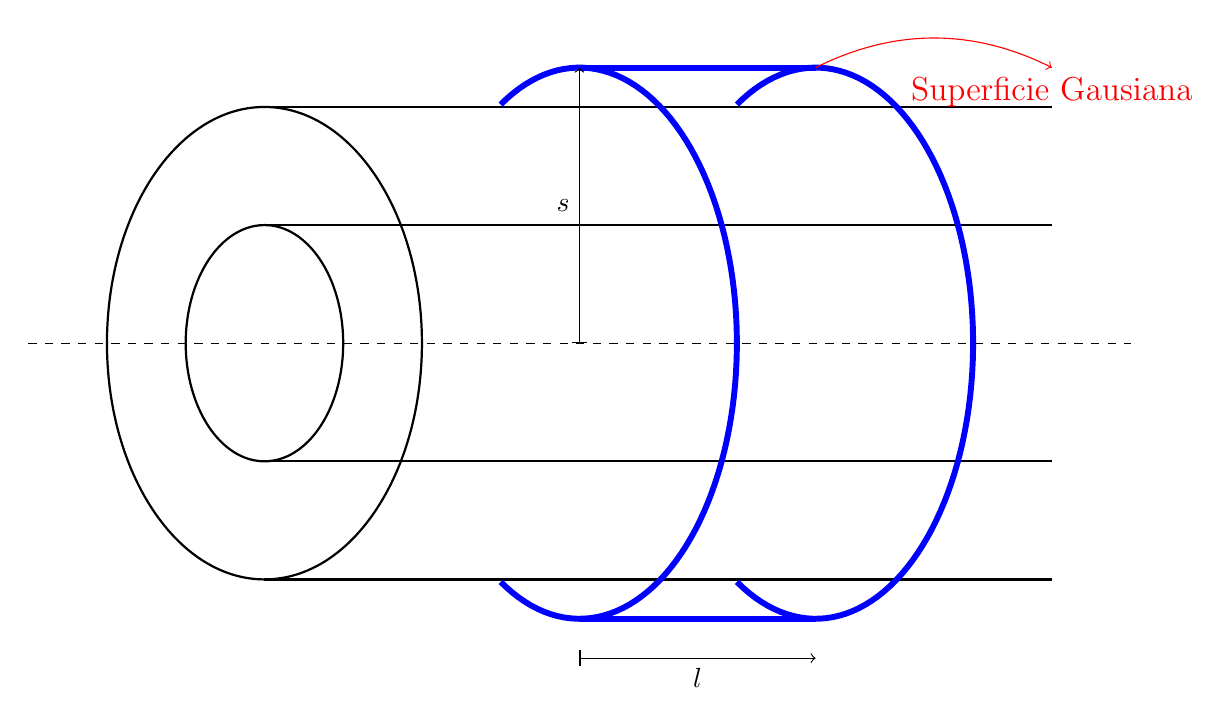
\begin{tikzpicture}
    % Outer cylinder (radius a)
    \draw[thick] (0,0) ellipse (2 and 3);
    \draw[thick] (0,0) ellipse (1 and 1.5);
    \draw[thick] (0,3) -- (10,3);
    \draw[thick] (0,1.5) -- (10,1.5);
    \draw[thick] (0,-1.5) -- (10,-1.5);
    \draw[thick] (0,-3) -- (10,-3);

    
    \draw[dashed](-3,0) -- (11,0);
    % cilindro de la parte interior  
    \draw[thick,blue, domain=120:-120, samples=100, variable=\t, line width=0.75mm] 
      plot ({2*cos(\t)+4}, {3.5*sin(\t)});
    
    \draw[thick,blue, domain=120:-120, samples=100, variable=\t, line width=0.75mm] 
      plot ({2*cos(\t)+7}, {3.5*sin(\t)});

    \draw[thick,blue, line width=0.75mm] (4,3.5) -- (7,3.5);
    \draw[thick,blue, line width=0.75mm] (4,-3.5) -- (7,-3.5);

    \draw[|->] (4,-4) -- (7,-4) node[midway,below] {$l$};
    \draw[|->,dash pattern=on 2pt off 0pt] (4,0) -- (4,3.5) node[midway,left] {$s$};

    \draw[->,red] (7,3.5) .. controls (8,4) and (9,4) .. (10,3.5) node[below,font=\large] {Superficie Gausiana};
\end{tikzpicture}
\end{document}